
% Default to the notebook output style

    


% Inherit from the specified cell style.




    
\documentclass[11pt]{article}

    
    
    \usepackage[T1]{fontenc}
    % Nicer default font (+ math font) than Computer Modern for most use cases
    \usepackage{mathpazo}

    % Basic figure setup, for now with no caption control since it's done
    % automatically by Pandoc (which extracts ![](path) syntax from Markdown).
    \usepackage{graphicx}
    % We will generate all images so they have a width \maxwidth. This means
    % that they will get their normal width if they fit onto the page, but
    % are scaled down if they would overflow the margins.
    \makeatletter
    \def\maxwidth{\ifdim\Gin@nat@width>\linewidth\linewidth
    \else\Gin@nat@width\fi}
    \makeatother
    \let\Oldincludegraphics\includegraphics
    % Set max figure width to be 80% of text width, for now hardcoded.
    \renewcommand{\includegraphics}[1]{\Oldincludegraphics[width=.8\maxwidth]{#1}}
    % Ensure that by default, figures have no caption (until we provide a
    % proper Figure object with a Caption API and a way to capture that
    % in the conversion process - todo).
    \usepackage{caption}
    \DeclareCaptionLabelFormat{nolabel}{}
    \captionsetup{labelformat=nolabel}

    \usepackage{adjustbox} % Used to constrain images to a maximum size 
    \usepackage{xcolor} % Allow colors to be defined
    \usepackage{enumerate} % Needed for markdown enumerations to work
    \usepackage{geometry} % Used to adjust the document margins
    \usepackage{amsmath} % Equations
    \usepackage{amssymb} % Equations
    \usepackage{textcomp} % defines textquotesingle
    % Hack from http://tex.stackexchange.com/a/47451/13684:
    \AtBeginDocument{%
        \def\PYZsq{\textquotesingle}% Upright quotes in Pygmentized code
    }
    \usepackage{upquote} % Upright quotes for verbatim code
    \usepackage{eurosym} % defines \euro
    \usepackage[mathletters]{ucs} % Extended unicode (utf-8) support
    \usepackage[utf8x]{inputenc} % Allow utf-8 characters in the tex document
    \usepackage{fancyvrb} % verbatim replacement that allows latex
    \usepackage{grffile} % extends the file name processing of package graphics 
                         % to support a larger range 
    % The hyperref package gives us a pdf with properly built
    % internal navigation ('pdf bookmarks' for the table of contents,
    % internal cross-reference links, web links for URLs, etc.)
    \usepackage{hyperref}
    \usepackage{longtable} % longtable support required by pandoc >1.10
    \usepackage{booktabs}  % table support for pandoc > 1.12.2
    \usepackage[inline]{enumitem} % IRkernel/repr support (it uses the enumerate* environment)
    \usepackage[normalem]{ulem} % ulem is needed to support strikethroughs (\sout)
                                % normalem makes italics be italics, not underlines
    

    
    
    % Colors for the hyperref package
    \definecolor{urlcolor}{rgb}{0,.145,.698}
    \definecolor{linkcolor}{rgb}{.71,0.21,0.01}
    \definecolor{citecolor}{rgb}{.12,.54,.11}

    % ANSI colors
    \definecolor{ansi-black}{HTML}{3E424D}
    \definecolor{ansi-black-intense}{HTML}{282C36}
    \definecolor{ansi-red}{HTML}{E75C58}
    \definecolor{ansi-red-intense}{HTML}{B22B31}
    \definecolor{ansi-green}{HTML}{00A250}
    \definecolor{ansi-green-intense}{HTML}{007427}
    \definecolor{ansi-yellow}{HTML}{DDB62B}
    \definecolor{ansi-yellow-intense}{HTML}{B27D12}
    \definecolor{ansi-blue}{HTML}{208FFB}
    \definecolor{ansi-blue-intense}{HTML}{0065CA}
    \definecolor{ansi-magenta}{HTML}{D160C4}
    \definecolor{ansi-magenta-intense}{HTML}{A03196}
    \definecolor{ansi-cyan}{HTML}{60C6C8}
    \definecolor{ansi-cyan-intense}{HTML}{258F8F}
    \definecolor{ansi-white}{HTML}{C5C1B4}
    \definecolor{ansi-white-intense}{HTML}{A1A6B2}

    % commands and environments needed by pandoc snippets
    % extracted from the output of `pandoc -s`
    \providecommand{\tightlist}{%
      \setlength{\itemsep}{0pt}\setlength{\parskip}{0pt}}
    \DefineVerbatimEnvironment{Highlighting}{Verbatim}{commandchars=\\\{\}}
    % Add ',fontsize=\small' for more characters per line
    \newenvironment{Shaded}{}{}
    \newcommand{\KeywordTok}[1]{\textcolor[rgb]{0.00,0.44,0.13}{\textbf{{#1}}}}
    \newcommand{\DataTypeTok}[1]{\textcolor[rgb]{0.56,0.13,0.00}{{#1}}}
    \newcommand{\DecValTok}[1]{\textcolor[rgb]{0.25,0.63,0.44}{{#1}}}
    \newcommand{\BaseNTok}[1]{\textcolor[rgb]{0.25,0.63,0.44}{{#1}}}
    \newcommand{\FloatTok}[1]{\textcolor[rgb]{0.25,0.63,0.44}{{#1}}}
    \newcommand{\CharTok}[1]{\textcolor[rgb]{0.25,0.44,0.63}{{#1}}}
    \newcommand{\StringTok}[1]{\textcolor[rgb]{0.25,0.44,0.63}{{#1}}}
    \newcommand{\CommentTok}[1]{\textcolor[rgb]{0.38,0.63,0.69}{\textit{{#1}}}}
    \newcommand{\OtherTok}[1]{\textcolor[rgb]{0.00,0.44,0.13}{{#1}}}
    \newcommand{\AlertTok}[1]{\textcolor[rgb]{1.00,0.00,0.00}{\textbf{{#1}}}}
    \newcommand{\FunctionTok}[1]{\textcolor[rgb]{0.02,0.16,0.49}{{#1}}}
    \newcommand{\RegionMarkerTok}[1]{{#1}}
    \newcommand{\ErrorTok}[1]{\textcolor[rgb]{1.00,0.00,0.00}{\textbf{{#1}}}}
    \newcommand{\NormalTok}[1]{{#1}}
    
    % Additional commands for more recent versions of Pandoc
    \newcommand{\ConstantTok}[1]{\textcolor[rgb]{0.53,0.00,0.00}{{#1}}}
    \newcommand{\SpecialCharTok}[1]{\textcolor[rgb]{0.25,0.44,0.63}{{#1}}}
    \newcommand{\VerbatimStringTok}[1]{\textcolor[rgb]{0.25,0.44,0.63}{{#1}}}
    \newcommand{\SpecialStringTok}[1]{\textcolor[rgb]{0.73,0.40,0.53}{{#1}}}
    \newcommand{\ImportTok}[1]{{#1}}
    \newcommand{\DocumentationTok}[1]{\textcolor[rgb]{0.73,0.13,0.13}{\textit{{#1}}}}
    \newcommand{\AnnotationTok}[1]{\textcolor[rgb]{0.38,0.63,0.69}{\textbf{\textit{{#1}}}}}
    \newcommand{\CommentVarTok}[1]{\textcolor[rgb]{0.38,0.63,0.69}{\textbf{\textit{{#1}}}}}
    \newcommand{\VariableTok}[1]{\textcolor[rgb]{0.10,0.09,0.49}{{#1}}}
    \newcommand{\ControlFlowTok}[1]{\textcolor[rgb]{0.00,0.44,0.13}{\textbf{{#1}}}}
    \newcommand{\OperatorTok}[1]{\textcolor[rgb]{0.40,0.40,0.40}{{#1}}}
    \newcommand{\BuiltInTok}[1]{{#1}}
    \newcommand{\ExtensionTok}[1]{{#1}}
    \newcommand{\PreprocessorTok}[1]{\textcolor[rgb]{0.74,0.48,0.00}{{#1}}}
    \newcommand{\AttributeTok}[1]{\textcolor[rgb]{0.49,0.56,0.16}{{#1}}}
    \newcommand{\InformationTok}[1]{\textcolor[rgb]{0.38,0.63,0.69}{\textbf{\textit{{#1}}}}}
    \newcommand{\WarningTok}[1]{\textcolor[rgb]{0.38,0.63,0.69}{\textbf{\textit{{#1}}}}}
    
    
    % Define a nice break command that doesn't care if a line doesn't already
    % exist.
    \def\br{\hspace*{\fill} \\* }
    % Math Jax compatability definitions
    \def\gt{>}
    \def\lt{<}
    % Document parameters
    \title{Oslo\_city\_bike\_EDA}
    
    
    

    % Pygments definitions
    
\makeatletter
\def\PY@reset{\let\PY@it=\relax \let\PY@bf=\relax%
    \let\PY@ul=\relax \let\PY@tc=\relax%
    \let\PY@bc=\relax \let\PY@ff=\relax}
\def\PY@tok#1{\csname PY@tok@#1\endcsname}
\def\PY@toks#1+{\ifx\relax#1\empty\else%
    \PY@tok{#1}\expandafter\PY@toks\fi}
\def\PY@do#1{\PY@bc{\PY@tc{\PY@ul{%
    \PY@it{\PY@bf{\PY@ff{#1}}}}}}}
\def\PY#1#2{\PY@reset\PY@toks#1+\relax+\PY@do{#2}}

\expandafter\def\csname PY@tok@w\endcsname{\def\PY@tc##1{\textcolor[rgb]{0.73,0.73,0.73}{##1}}}
\expandafter\def\csname PY@tok@c\endcsname{\let\PY@it=\textit\def\PY@tc##1{\textcolor[rgb]{0.25,0.50,0.50}{##1}}}
\expandafter\def\csname PY@tok@cp\endcsname{\def\PY@tc##1{\textcolor[rgb]{0.74,0.48,0.00}{##1}}}
\expandafter\def\csname PY@tok@k\endcsname{\let\PY@bf=\textbf\def\PY@tc##1{\textcolor[rgb]{0.00,0.50,0.00}{##1}}}
\expandafter\def\csname PY@tok@kp\endcsname{\def\PY@tc##1{\textcolor[rgb]{0.00,0.50,0.00}{##1}}}
\expandafter\def\csname PY@tok@kt\endcsname{\def\PY@tc##1{\textcolor[rgb]{0.69,0.00,0.25}{##1}}}
\expandafter\def\csname PY@tok@o\endcsname{\def\PY@tc##1{\textcolor[rgb]{0.40,0.40,0.40}{##1}}}
\expandafter\def\csname PY@tok@ow\endcsname{\let\PY@bf=\textbf\def\PY@tc##1{\textcolor[rgb]{0.67,0.13,1.00}{##1}}}
\expandafter\def\csname PY@tok@nb\endcsname{\def\PY@tc##1{\textcolor[rgb]{0.00,0.50,0.00}{##1}}}
\expandafter\def\csname PY@tok@nf\endcsname{\def\PY@tc##1{\textcolor[rgb]{0.00,0.00,1.00}{##1}}}
\expandafter\def\csname PY@tok@nc\endcsname{\let\PY@bf=\textbf\def\PY@tc##1{\textcolor[rgb]{0.00,0.00,1.00}{##1}}}
\expandafter\def\csname PY@tok@nn\endcsname{\let\PY@bf=\textbf\def\PY@tc##1{\textcolor[rgb]{0.00,0.00,1.00}{##1}}}
\expandafter\def\csname PY@tok@ne\endcsname{\let\PY@bf=\textbf\def\PY@tc##1{\textcolor[rgb]{0.82,0.25,0.23}{##1}}}
\expandafter\def\csname PY@tok@nv\endcsname{\def\PY@tc##1{\textcolor[rgb]{0.10,0.09,0.49}{##1}}}
\expandafter\def\csname PY@tok@no\endcsname{\def\PY@tc##1{\textcolor[rgb]{0.53,0.00,0.00}{##1}}}
\expandafter\def\csname PY@tok@nl\endcsname{\def\PY@tc##1{\textcolor[rgb]{0.63,0.63,0.00}{##1}}}
\expandafter\def\csname PY@tok@ni\endcsname{\let\PY@bf=\textbf\def\PY@tc##1{\textcolor[rgb]{0.60,0.60,0.60}{##1}}}
\expandafter\def\csname PY@tok@na\endcsname{\def\PY@tc##1{\textcolor[rgb]{0.49,0.56,0.16}{##1}}}
\expandafter\def\csname PY@tok@nt\endcsname{\let\PY@bf=\textbf\def\PY@tc##1{\textcolor[rgb]{0.00,0.50,0.00}{##1}}}
\expandafter\def\csname PY@tok@nd\endcsname{\def\PY@tc##1{\textcolor[rgb]{0.67,0.13,1.00}{##1}}}
\expandafter\def\csname PY@tok@s\endcsname{\def\PY@tc##1{\textcolor[rgb]{0.73,0.13,0.13}{##1}}}
\expandafter\def\csname PY@tok@sd\endcsname{\let\PY@it=\textit\def\PY@tc##1{\textcolor[rgb]{0.73,0.13,0.13}{##1}}}
\expandafter\def\csname PY@tok@si\endcsname{\let\PY@bf=\textbf\def\PY@tc##1{\textcolor[rgb]{0.73,0.40,0.53}{##1}}}
\expandafter\def\csname PY@tok@se\endcsname{\let\PY@bf=\textbf\def\PY@tc##1{\textcolor[rgb]{0.73,0.40,0.13}{##1}}}
\expandafter\def\csname PY@tok@sr\endcsname{\def\PY@tc##1{\textcolor[rgb]{0.73,0.40,0.53}{##1}}}
\expandafter\def\csname PY@tok@ss\endcsname{\def\PY@tc##1{\textcolor[rgb]{0.10,0.09,0.49}{##1}}}
\expandafter\def\csname PY@tok@sx\endcsname{\def\PY@tc##1{\textcolor[rgb]{0.00,0.50,0.00}{##1}}}
\expandafter\def\csname PY@tok@m\endcsname{\def\PY@tc##1{\textcolor[rgb]{0.40,0.40,0.40}{##1}}}
\expandafter\def\csname PY@tok@gh\endcsname{\let\PY@bf=\textbf\def\PY@tc##1{\textcolor[rgb]{0.00,0.00,0.50}{##1}}}
\expandafter\def\csname PY@tok@gu\endcsname{\let\PY@bf=\textbf\def\PY@tc##1{\textcolor[rgb]{0.50,0.00,0.50}{##1}}}
\expandafter\def\csname PY@tok@gd\endcsname{\def\PY@tc##1{\textcolor[rgb]{0.63,0.00,0.00}{##1}}}
\expandafter\def\csname PY@tok@gi\endcsname{\def\PY@tc##1{\textcolor[rgb]{0.00,0.63,0.00}{##1}}}
\expandafter\def\csname PY@tok@gr\endcsname{\def\PY@tc##1{\textcolor[rgb]{1.00,0.00,0.00}{##1}}}
\expandafter\def\csname PY@tok@ge\endcsname{\let\PY@it=\textit}
\expandafter\def\csname PY@tok@gs\endcsname{\let\PY@bf=\textbf}
\expandafter\def\csname PY@tok@gp\endcsname{\let\PY@bf=\textbf\def\PY@tc##1{\textcolor[rgb]{0.00,0.00,0.50}{##1}}}
\expandafter\def\csname PY@tok@go\endcsname{\def\PY@tc##1{\textcolor[rgb]{0.53,0.53,0.53}{##1}}}
\expandafter\def\csname PY@tok@gt\endcsname{\def\PY@tc##1{\textcolor[rgb]{0.00,0.27,0.87}{##1}}}
\expandafter\def\csname PY@tok@err\endcsname{\def\PY@bc##1{\setlength{\fboxsep}{0pt}\fcolorbox[rgb]{1.00,0.00,0.00}{1,1,1}{\strut ##1}}}
\expandafter\def\csname PY@tok@kc\endcsname{\let\PY@bf=\textbf\def\PY@tc##1{\textcolor[rgb]{0.00,0.50,0.00}{##1}}}
\expandafter\def\csname PY@tok@kd\endcsname{\let\PY@bf=\textbf\def\PY@tc##1{\textcolor[rgb]{0.00,0.50,0.00}{##1}}}
\expandafter\def\csname PY@tok@kn\endcsname{\let\PY@bf=\textbf\def\PY@tc##1{\textcolor[rgb]{0.00,0.50,0.00}{##1}}}
\expandafter\def\csname PY@tok@kr\endcsname{\let\PY@bf=\textbf\def\PY@tc##1{\textcolor[rgb]{0.00,0.50,0.00}{##1}}}
\expandafter\def\csname PY@tok@bp\endcsname{\def\PY@tc##1{\textcolor[rgb]{0.00,0.50,0.00}{##1}}}
\expandafter\def\csname PY@tok@fm\endcsname{\def\PY@tc##1{\textcolor[rgb]{0.00,0.00,1.00}{##1}}}
\expandafter\def\csname PY@tok@vc\endcsname{\def\PY@tc##1{\textcolor[rgb]{0.10,0.09,0.49}{##1}}}
\expandafter\def\csname PY@tok@vg\endcsname{\def\PY@tc##1{\textcolor[rgb]{0.10,0.09,0.49}{##1}}}
\expandafter\def\csname PY@tok@vi\endcsname{\def\PY@tc##1{\textcolor[rgb]{0.10,0.09,0.49}{##1}}}
\expandafter\def\csname PY@tok@vm\endcsname{\def\PY@tc##1{\textcolor[rgb]{0.10,0.09,0.49}{##1}}}
\expandafter\def\csname PY@tok@sa\endcsname{\def\PY@tc##1{\textcolor[rgb]{0.73,0.13,0.13}{##1}}}
\expandafter\def\csname PY@tok@sb\endcsname{\def\PY@tc##1{\textcolor[rgb]{0.73,0.13,0.13}{##1}}}
\expandafter\def\csname PY@tok@sc\endcsname{\def\PY@tc##1{\textcolor[rgb]{0.73,0.13,0.13}{##1}}}
\expandafter\def\csname PY@tok@dl\endcsname{\def\PY@tc##1{\textcolor[rgb]{0.73,0.13,0.13}{##1}}}
\expandafter\def\csname PY@tok@s2\endcsname{\def\PY@tc##1{\textcolor[rgb]{0.73,0.13,0.13}{##1}}}
\expandafter\def\csname PY@tok@sh\endcsname{\def\PY@tc##1{\textcolor[rgb]{0.73,0.13,0.13}{##1}}}
\expandafter\def\csname PY@tok@s1\endcsname{\def\PY@tc##1{\textcolor[rgb]{0.73,0.13,0.13}{##1}}}
\expandafter\def\csname PY@tok@mb\endcsname{\def\PY@tc##1{\textcolor[rgb]{0.40,0.40,0.40}{##1}}}
\expandafter\def\csname PY@tok@mf\endcsname{\def\PY@tc##1{\textcolor[rgb]{0.40,0.40,0.40}{##1}}}
\expandafter\def\csname PY@tok@mh\endcsname{\def\PY@tc##1{\textcolor[rgb]{0.40,0.40,0.40}{##1}}}
\expandafter\def\csname PY@tok@mi\endcsname{\def\PY@tc##1{\textcolor[rgb]{0.40,0.40,0.40}{##1}}}
\expandafter\def\csname PY@tok@il\endcsname{\def\PY@tc##1{\textcolor[rgb]{0.40,0.40,0.40}{##1}}}
\expandafter\def\csname PY@tok@mo\endcsname{\def\PY@tc##1{\textcolor[rgb]{0.40,0.40,0.40}{##1}}}
\expandafter\def\csname PY@tok@ch\endcsname{\let\PY@it=\textit\def\PY@tc##1{\textcolor[rgb]{0.25,0.50,0.50}{##1}}}
\expandafter\def\csname PY@tok@cm\endcsname{\let\PY@it=\textit\def\PY@tc##1{\textcolor[rgb]{0.25,0.50,0.50}{##1}}}
\expandafter\def\csname PY@tok@cpf\endcsname{\let\PY@it=\textit\def\PY@tc##1{\textcolor[rgb]{0.25,0.50,0.50}{##1}}}
\expandafter\def\csname PY@tok@c1\endcsname{\let\PY@it=\textit\def\PY@tc##1{\textcolor[rgb]{0.25,0.50,0.50}{##1}}}
\expandafter\def\csname PY@tok@cs\endcsname{\let\PY@it=\textit\def\PY@tc##1{\textcolor[rgb]{0.25,0.50,0.50}{##1}}}

\def\PYZbs{\char`\\}
\def\PYZus{\char`\_}
\def\PYZob{\char`\{}
\def\PYZcb{\char`\}}
\def\PYZca{\char`\^}
\def\PYZam{\char`\&}
\def\PYZlt{\char`\<}
\def\PYZgt{\char`\>}
\def\PYZsh{\char`\#}
\def\PYZpc{\char`\%}
\def\PYZdl{\char`\$}
\def\PYZhy{\char`\-}
\def\PYZsq{\char`\'}
\def\PYZdq{\char`\"}
\def\PYZti{\char`\~}
% for compatibility with earlier versions
\def\PYZat{@}
\def\PYZlb{[}
\def\PYZrb{]}
\makeatother


    % Exact colors from NB
    \definecolor{incolor}{rgb}{0.0, 0.0, 0.5}
    \definecolor{outcolor}{rgb}{0.545, 0.0, 0.0}



    
    % Prevent overflowing lines due to hard-to-break entities
    \sloppy 
    % Setup hyperref package
    \hypersetup{
      breaklinks=true,  % so long urls are correctly broken across lines
      colorlinks=true,
      urlcolor=urlcolor,
      linkcolor=linkcolor,
      citecolor=citecolor,
      }
    % Slightly bigger margins than the latex defaults
    
    \geometry{verbose,tmargin=1in,bmargin=1in,lmargin=1in,rmargin=1in}
    
    

    \begin{document}
    
    
    \maketitle
    
    

    
    \subsection{Oslo city bike data exploration
analysis}\label{oslo-city-bike-data-exploration-analysis}

    In Oslo, the capital of Norway, bikes can be rented and returned at
(presently) 230 locations in the city. Riding a bike to get around the
city is very popular during the summer time. Below I do some exploratory
data analysis from the data I got from
https://developer.oslobysykkel.no/data and https://yr.no.

This notebook is for my learning and everyone is free to use the code.
Please also give suggestions to improve the code.

The pic below taken from https://visitoslo.com

    \begin{figure}
\centering
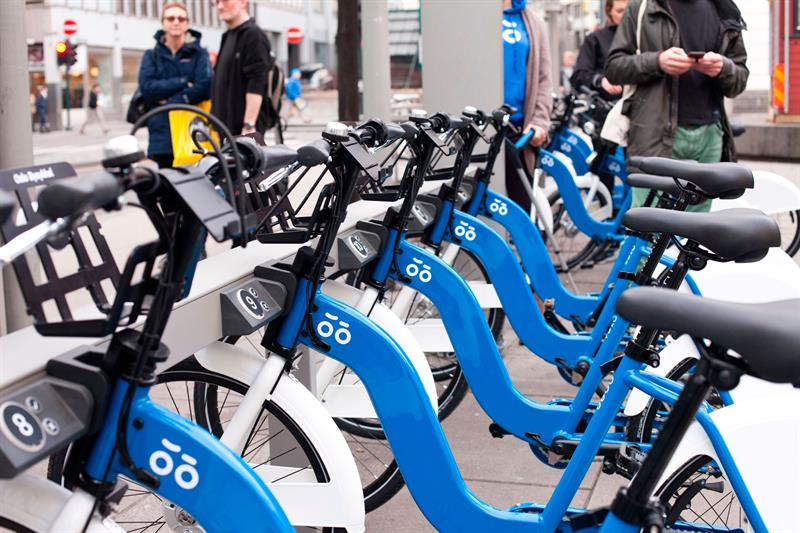
\includegraphics{bike_pic.jpeg}
\caption{title}
\end{figure}

    \subsection{Imorting modules}\label{imorting-modules}

    \begin{Verbatim}[commandchars=\\\{\}]
{\color{incolor}In [{\color{incolor}181}]:} \PY{k+kn}{import} \PY{n+nn}{pandas} \PY{k}{as} \PY{n+nn}{pd}
          \PY{k+kn}{import} \PY{n+nn}{numpy} \PY{k}{as} \PY{n+nn}{np}
          \PY{k+kn}{import} \PY{n+nn}{seaborn} \PY{k}{as} \PY{n+nn}{sns}
          \PY{k+kn}{import} \PY{n+nn}{matplotlib}\PY{n+nn}{.}\PY{n+nn}{pyplot} \PY{k}{as} \PY{n+nn}{plt}
          \PY{o}{\PYZpc{}}\PY{k}{matplotlib} inline
          \PY{n}{sns}\PY{o}{.}\PY{n}{set}\PY{p}{(}\PY{n}{color\PYZus{}codes}\PY{o}{=}\PY{k+kc}{True}\PY{p}{)}
          
          \PY{k+kn}{from} \PY{n+nn}{sklearn}\PY{n+nn}{.}\PY{n+nn}{linear\PYZus{}model} \PY{k}{import} \PY{n}{LinearRegression}
          \PY{k+kn}{from} \PY{n+nn}{sklearn}\PY{n+nn}{.}\PY{n+nn}{model\PYZus{}selection} \PY{k}{import} \PY{n}{train\PYZus{}test\PYZus{}split}
          \PY{k+kn}{from} \PY{n+nn}{sklearn}\PY{n+nn}{.}\PY{n+nn}{metrics} \PY{k}{import} \PY{n}{mean\PYZus{}squared\PYZus{}error}
          \PY{k+kn}{from} \PY{n+nn}{math} \PY{k}{import} \PY{n}{sqrt}
          
          \PY{k+kn}{import} \PY{n+nn}{json}
          \PY{k+kn}{from} \PY{n+nn}{pandas}\PY{n+nn}{.}\PY{n+nn}{io}\PY{n+nn}{.}\PY{n+nn}{json} \PY{k}{import} \PY{n}{json\PYZus{}normalize}
          
          \PY{k+kn}{import} \PY{n+nn}{datetime}
          \PY{k+kn}{import} \PY{n+nn}{calendar}
          
          \PY{k+kn}{import} \PY{n+nn}{gmaps}
          
          \PY{k+kn}{import} \PY{n+nn}{folium}
\end{Verbatim}


    \subsection{Loading of data}\label{loading-of-data}

    \begin{Verbatim}[commandchars=\\\{\}]
{\color{incolor}In [{\color{incolor}7}]:} \PY{c+c1}{\PYZsh{}Loading of bike data}
        \PY{n}{april18}\PY{o}{=}\PY{n}{pd}\PY{o}{.}\PY{n}{read\PYZus{}csv}\PY{p}{(}\PY{l+s+s1}{\PYZsq{}}\PY{l+s+s1}{trips\PYZhy{}2018.4.1\PYZhy{}2018.4.30.csv}\PY{l+s+s1}{\PYZsq{}}\PY{p}{,}\PY{n}{parse\PYZus{}dates}\PY{o}{=}\PY{p}{[}\PY{l+s+s1}{\PYZsq{}}\PY{l+s+s1}{Start time}\PY{l+s+s1}{\PYZsq{}}\PY{p}{,}\PY{l+s+s1}{\PYZsq{}}\PY{l+s+s1}{End time}\PY{l+s+s1}{\PYZsq{}}\PY{p}{]}\PY{p}{)}
        \PY{n}{may18}\PY{o}{=}\PY{n}{pd}\PY{o}{.}\PY{n}{read\PYZus{}csv}\PY{p}{(}\PY{l+s+s1}{\PYZsq{}}\PY{l+s+s1}{trips\PYZhy{}2018.5.1\PYZhy{}2018.5.31.csv}\PY{l+s+s1}{\PYZsq{}}\PY{p}{,}\PY{n}{parse\PYZus{}dates}\PY{o}{=}\PY{p}{[}\PY{l+s+s1}{\PYZsq{}}\PY{l+s+s1}{Start time}\PY{l+s+s1}{\PYZsq{}}\PY{p}{,}\PY{l+s+s1}{\PYZsq{}}\PY{l+s+s1}{End time}\PY{l+s+s1}{\PYZsq{}}\PY{p}{]}\PY{p}{)}
        \PY{n}{june18}\PY{o}{=}\PY{n}{pd}\PY{o}{.}\PY{n}{read\PYZus{}csv}\PY{p}{(}\PY{l+s+s1}{\PYZsq{}}\PY{l+s+s1}{trips\PYZhy{}2018.6.1\PYZhy{}2018.6.30.csv}\PY{l+s+s1}{\PYZsq{}}\PY{p}{,}\PY{n}{parse\PYZus{}dates}\PY{o}{=}\PY{p}{[}\PY{l+s+s1}{\PYZsq{}}\PY{l+s+s1}{Start time}\PY{l+s+s1}{\PYZsq{}}\PY{p}{,}\PY{l+s+s1}{\PYZsq{}}\PY{l+s+s1}{End time}\PY{l+s+s1}{\PYZsq{}}\PY{p}{]}\PY{p}{)}
        \PY{n}{july18}\PY{o}{=}\PY{n}{pd}\PY{o}{.}\PY{n}{read\PYZus{}csv}\PY{p}{(}\PY{l+s+s1}{\PYZsq{}}\PY{l+s+s1}{trips\PYZhy{}2018.7.1\PYZhy{}2018.7.31.csv}\PY{l+s+s1}{\PYZsq{}}\PY{p}{,}\PY{n}{parse\PYZus{}dates}\PY{o}{=}\PY{p}{[}\PY{l+s+s1}{\PYZsq{}}\PY{l+s+s1}{Start time}\PY{l+s+s1}{\PYZsq{}}\PY{p}{,}\PY{l+s+s1}{\PYZsq{}}\PY{l+s+s1}{End time}\PY{l+s+s1}{\PYZsq{}}\PY{p}{]}\PY{p}{)}
        
        \PY{n}{july17}\PY{o}{=}\PY{n}{pd}\PY{o}{.}\PY{n}{read\PYZus{}csv}\PY{p}{(}\PY{l+s+s1}{\PYZsq{}}\PY{l+s+s1}{trips\PYZhy{}2017.7.1\PYZhy{}2017.7.31.csv}\PY{l+s+s1}{\PYZsq{}}\PY{p}{,}\PY{n}{parse\PYZus{}dates}\PY{o}{=}\PY{p}{[}\PY{l+s+s1}{\PYZsq{}}\PY{l+s+s1}{Start time}\PY{l+s+s1}{\PYZsq{}}\PY{p}{,}\PY{l+s+s1}{\PYZsq{}}\PY{l+s+s1}{End time}\PY{l+s+s1}{\PYZsq{}}\PY{p}{]}\PY{p}{)}
        \PY{n}{july16}\PY{o}{=}\PY{n}{pd}\PY{o}{.}\PY{n}{read\PYZus{}csv}\PY{p}{(}\PY{l+s+s1}{\PYZsq{}}\PY{l+s+s1}{trips\PYZhy{}2016.7.1\PYZhy{}2016.7.31.csv}\PY{l+s+s1}{\PYZsq{}}\PY{p}{,}\PY{n}{parse\PYZus{}dates}\PY{o}{=}\PY{p}{[}\PY{l+s+s1}{\PYZsq{}}\PY{l+s+s1}{Start time}\PY{l+s+s1}{\PYZsq{}}\PY{p}{,}\PY{l+s+s1}{\PYZsq{}}\PY{l+s+s1}{End time}\PY{l+s+s1}{\PYZsq{}}\PY{p}{]}\PY{p}{)}
\end{Verbatim}


    \begin{Verbatim}[commandchars=\\\{\}]
{\color{incolor}In [{\color{incolor}8}]:} \PY{c+c1}{\PYZsh{} Let\PYZsq{}s look at the columns}
        \PY{n}{july18}\PY{o}{.}\PY{n}{head}\PY{p}{(}\PY{p}{)}
\end{Verbatim}


\begin{Verbatim}[commandchars=\\\{\}]
{\color{outcolor}Out[{\color{outcolor}8}]:}    Start station          Start time  End station            End time
        0            207 2018-07-01 04:00:15          177 2018-07-01 04:06:37
        1            189 2018-07-01 04:00:34          203 2018-07-01 04:05:38
        2            470 2018-07-01 04:00:38          247 2018-07-01 04:07:39
        3            246 2018-07-01 04:00:46          242 2018-07-01 04:11:59
        4            222 2018-07-01 04:00:55          247 2018-07-01 04:08:52
\end{Verbatim}
            
    \begin{Verbatim}[commandchars=\\\{\}]
{\color{incolor}In [{\color{incolor}26}]:} \PY{c+c1}{\PYZsh{}Combine data for all the available months of 2018}
         \PY{n}{dfcomb}\PY{o}{=}\PY{n}{pd}\PY{o}{.}\PY{n}{concat}\PY{p}{(}\PY{p}{[}\PY{n}{april18}\PY{p}{,}\PY{n}{may18}\PY{p}{,}\PY{n}{june18}\PY{p}{,}\PY{n}{july18}\PY{p}{]}\PY{p}{)}
\end{Verbatim}


    \begin{Verbatim}[commandchars=\\\{\}]
{\color{incolor}In [{\color{incolor}27}]:} \PY{c+c1}{\PYZsh{}Let\PYZsq{}s add a column for the duration of the rented period. The period in minutes.}
         \PY{n}{dfcomb}\PY{p}{[}\PY{l+s+s1}{\PYZsq{}}\PY{l+s+s1}{duration}\PY{l+s+s1}{\PYZsq{}}\PY{p}{]}\PY{o}{=}\PY{p}{(}\PY{p}{(}\PY{n}{dfcomb}\PY{p}{[}\PY{l+s+s1}{\PYZsq{}}\PY{l+s+s1}{End time}\PY{l+s+s1}{\PYZsq{}}\PY{p}{]}\PY{o}{\PYZhy{}}\PY{n}{dfcomb}\PY{p}{[}\PY{l+s+s1}{\PYZsq{}}\PY{l+s+s1}{Start time}\PY{l+s+s1}{\PYZsq{}}\PY{p}{]}\PY{p}{)}\PY{o}{.}\PY{n}{dt}\PY{o}{.}\PY{n}{total\PYZus{}seconds}\PY{p}{(}\PY{p}{)}\PY{p}{)}\PY{o}{/}\PY{l+m+mf}{60.0}
\end{Verbatim}


    \begin{Verbatim}[commandchars=\\\{\}]
{\color{incolor}In [{\color{incolor}28}]:} \PY{n}{dfcomb}\PY{o}{.}\PY{n}{describe}\PY{p}{(}\PY{p}{)}
\end{Verbatim}


\begin{Verbatim}[commandchars=\\\{\}]
{\color{outcolor}Out[{\color{outcolor}28}]:}        Start station   End station      duration
         count   1.686706e+06  1.686706e+06  1.686706e+06
         mean    2.758795e+02  2.764166e+02  1.585371e+01
         std     8.208443e+01  8.199220e+01  1.176022e+02
         min     1.570000e+02  1.570000e+02 -3.520000e+01
         25\%     2.070000e+02  2.080000e+02  5.550000e+00
         50\%     2.620000e+02  2.620000e+02  9.266667e+00
         75\%     3.450000e+02  3.450000e+02  1.568333e+01
         max     4.860000e+02  4.860000e+02  3.025447e+04
\end{Verbatim}
            
    We can see from the above output that there is negative duration for
some data entries and the maximum period is nearly 20 days! Let's now
clean the data

    \begin{Verbatim}[commandchars=\\\{\}]
{\color{incolor}In [{\color{incolor}29}]:} \PY{n}{cutoffduration}\PY{o}{=}\PY{l+m+mf}{200.0} \PY{c+c1}{\PYZsh{} value of duration above which the data is ignored}
         \PY{n}{dfcomb}\PY{o}{=}\PY{n}{dfcomb}\PY{o}{.}\PY{n}{drop}\PY{p}{(}\PY{n}{dfcomb}\PY{p}{[}\PY{p}{(}\PY{n}{dfcomb}\PY{p}{[}\PY{l+s+s1}{\PYZsq{}}\PY{l+s+s1}{duration}\PY{l+s+s1}{\PYZsq{}}\PY{p}{]}\PY{o}{\PYZgt{}}\PY{n}{cutoffduration}\PY{p}{)}\PY{o}{|}\PY{p}{(}\PY{n}{dfcomb}\PY{p}{[}\PY{l+s+s1}{\PYZsq{}}\PY{l+s+s1}{duration}\PY{l+s+s1}{\PYZsq{}}\PY{p}{]}\PY{o}{\PYZlt{}}\PY{l+m+mi}{0}\PY{p}{)}\PY{p}{]}\PY{o}{.}\PY{n}{index}\PY{p}{)}
\end{Verbatim}


    Let's also drop the points when the start and end point are the same and
the duration is less than one minute. These are typically the instances
when a user decided not to take the bike.

    \begin{Verbatim}[commandchars=\\\{\}]
{\color{incolor}In [{\color{incolor}129}]:} \PY{n}{dfcomb}\PY{o}{=}\PY{n}{dfcomb}\PY{o}{.}\PY{n}{drop}\PY{p}{(}\PY{n}{dfcomb}\PY{p}{[}\PY{p}{(}\PY{n}{dfcomb}\PY{p}{[}\PY{l+s+s1}{\PYZsq{}}\PY{l+s+s1}{duration}\PY{l+s+s1}{\PYZsq{}}\PY{p}{]}\PY{o}{\PYZlt{}}\PY{l+m+mi}{1}\PY{p}{)}\PY{o}{\PYZam{}}\PY{p}{(}\PY{n}{dfcomb}\PY{p}{[}\PY{l+s+s1}{\PYZsq{}}\PY{l+s+s1}{Start station}\PY{l+s+s1}{\PYZsq{}}\PY{p}{]}\PY{o}{==}\PY{n}{dfcomb}\PY{p}{[}\PY{l+s+s1}{\PYZsq{}}\PY{l+s+s1}{End station}\PY{l+s+s1}{\PYZsq{}}\PY{p}{]}\PY{p}{)}\PY{p}{]}\PY{o}{.}\PY{n}{index}\PY{p}{)}
\end{Verbatim}


    \begin{Verbatim}[commandchars=\\\{\}]
{\color{incolor}In [{\color{incolor}130}]:} \PY{n}{dfcomb}\PY{o}{.}\PY{n}{describe}\PY{p}{(}\PY{p}{)}
\end{Verbatim}


\begin{Verbatim}[commandchars=\\\{\}]
{\color{outcolor}Out[{\color{outcolor}130}]:}            duration          Hour
          count  1.490987e+06  1.490987e+06
          mean   1.333106e+01  1.594291e+01
          std    1.335296e+01  4.501422e+00
          min    2.500000e-01  2.133333e+00
          25\%    5.866667e+00  1.290000e+01
          50\%    9.516667e+00  1.653333e+01
          75\%    1.591667e+01  1.931667e+01
          max    1.999833e+02  2.598333e+01
\end{Verbatim}
            
    \begin{Verbatim}[commandchars=\\\{\}]
{\color{incolor}In [{\color{incolor}32}]:} \PY{c+c1}{\PYZsh{} Let\PYZsq{}s plot to see if the cutoff of 200 is justified}
         \PY{n}{sns}\PY{o}{.}\PY{n}{distplot}\PY{p}{(}\PY{n}{dfcomb}\PY{p}{[}\PY{l+s+s1}{\PYZsq{}}\PY{l+s+s1}{duration}\PY{l+s+s1}{\PYZsq{}}\PY{p}{]}\PY{p}{)}
\end{Verbatim}


\begin{Verbatim}[commandchars=\\\{\}]
{\color{outcolor}Out[{\color{outcolor}32}]:} <matplotlib.axes.\_subplots.AxesSubplot at 0x1110c2588>
\end{Verbatim}
            
    \begin{center}
    \adjustimage{max size={0.9\linewidth}{0.9\paperheight}}{output_16_1.png}
    \end{center}
    { \hspace*{\fill} \\}
    
    A Chi-squared distribution

    \begin{Verbatim}[commandchars=\\\{\}]
{\color{incolor}In [{\color{incolor}33}]:} \PY{n}{sns}\PY{o}{.}\PY{n}{boxplot}\PY{p}{(}\PY{n}{dfcomb}\PY{p}{[}\PY{l+s+s1}{\PYZsq{}}\PY{l+s+s1}{duration}\PY{l+s+s1}{\PYZsq{}}\PY{p}{]}\PY{p}{[}\PY{n}{dfcomb}\PY{p}{[}\PY{l+s+s1}{\PYZsq{}}\PY{l+s+s1}{duration}\PY{l+s+s1}{\PYZsq{}}\PY{p}{]}\PY{o}{\PYZlt{}}\PY{l+m+mf}{1000.0}\PY{p}{]}\PY{p}{)}
\end{Verbatim}


\begin{Verbatim}[commandchars=\\\{\}]
{\color{outcolor}Out[{\color{outcolor}33}]:} <matplotlib.axes.\_subplots.AxesSubplot at 0x110de5f98>
\end{Verbatim}
            
    \begin{center}
    \adjustimage{max size={0.9\linewidth}{0.9\paperheight}}{output_18_1.png}
    \end{center}
    { \hspace*{\fill} \\}
    
    \begin{Verbatim}[commandchars=\\\{\}]
{\color{incolor}In [{\color{incolor}38}]:} \PY{n}{dfcomb}\PY{p}{[}\PY{l+s+s1}{\PYZsq{}}\PY{l+s+s1}{Date}\PY{l+s+s1}{\PYZsq{}}\PY{p}{]}\PY{o}{=} \PY{n}{dfcomb}\PY{p}{[}\PY{l+s+s1}{\PYZsq{}}\PY{l+s+s1}{Start time}\PY{l+s+s1}{\PYZsq{}}\PY{p}{]}\PY{o}{.}\PY{n}{dt}\PY{o}{.}\PY{n}{date}
\end{Verbatim}


    \begin{Verbatim}[commandchars=\\\{\}]
{\color{incolor}In [{\color{incolor}49}]:} \PY{n}{dfcomb}\PY{p}{[}\PY{l+s+s1}{\PYZsq{}}\PY{l+s+s1}{Month}\PY{l+s+s1}{\PYZsq{}}\PY{p}{]}\PY{o}{=} \PY{p}{(}\PY{n}{dfcomb}\PY{p}{[}\PY{l+s+s1}{\PYZsq{}}\PY{l+s+s1}{Start time}\PY{l+s+s1}{\PYZsq{}}\PY{p}{]}\PY{o}{.}\PY{n}{dt}\PY{o}{.}\PY{n}{month}\PY{p}{)}\PY{o}{.}\PY{n}{apply}\PY{p}{(}\PY{k}{lambda} \PY{n}{x}\PY{p}{:} \PY{n}{calendar}\PY{o}{.}\PY{n}{month\PYZus{}abbr}\PY{p}{[}\PY{n}{x}\PY{p}{]}\PY{p}{)}
         \PY{n}{dfcomb}\PY{p}{[}\PY{l+s+s1}{\PYZsq{}}\PY{l+s+s1}{Month}\PY{l+s+s1}{\PYZsq{}}\PY{p}{]}\PY{o}{.}\PY{n}{head}\PY{p}{(}\PY{p}{)}
\end{Verbatim}


\begin{Verbatim}[commandchars=\\\{\}]
{\color{outcolor}Out[{\color{outcolor}49}]:} 0    Apr
         1    Apr
         2    Apr
         3    Apr
         4    Apr
         Name: Month, dtype: object
\end{Verbatim}
            
    \begin{Verbatim}[commandchars=\\\{\}]
{\color{incolor}In [{\color{incolor}117}]:} \PY{n}{dfcomb}\PY{p}{[}\PY{l+s+s1}{\PYZsq{}}\PY{l+s+s1}{Hour}\PY{l+s+s1}{\PYZsq{}}\PY{p}{]}\PY{o}{=} \PY{l+m+mi}{2}\PY{o}{+} \PY{n}{dfcomb}\PY{p}{[}\PY{l+s+s1}{\PYZsq{}}\PY{l+s+s1}{Start time}\PY{l+s+s1}{\PYZsq{}}\PY{p}{]}\PY{o}{.}\PY{n}{dt}\PY{o}{.}\PY{n}{hour} \PY{o}{+}\PY{n}{dfcomb}\PY{p}{[}\PY{l+s+s1}{\PYZsq{}}\PY{l+s+s1}{Start time}\PY{l+s+s1}{\PYZsq{}}\PY{p}{]}\PY{o}{.}\PY{n}{dt}\PY{o}{.}\PY{n}{minute}\PY{o}{/}\PY{l+m+mf}{60.0}
          \PY{c+c1}{\PYZsh{} The 2 is added to convert to CEST}
          
          \PY{c+c1}{\PYZsh{}dfcomb[\PYZsq{}Minute\PYZsq{}]= dfcomb[\PYZsq{}Start time\PYZsq{}].dt.minute}
\end{Verbatim}


    \begin{Verbatim}[commandchars=\\\{\}]
{\color{incolor}In [{\color{incolor}115}]:} \PY{n}{dfcomb}\PY{p}{[}\PY{l+s+s1}{\PYZsq{}}\PY{l+s+s1}{Day}\PY{l+s+s1}{\PYZsq{}}\PY{p}{]}\PY{o}{=} \PY{n}{dfcomb}\PY{p}{[}\PY{l+s+s1}{\PYZsq{}}\PY{l+s+s1}{Start time}\PY{l+s+s1}{\PYZsq{}}\PY{p}{]}\PY{o}{.}\PY{n}{dt}\PY{o}{.}\PY{n}{weekday\PYZus{}name}
\end{Verbatim}


    \begin{Verbatim}[commandchars=\\\{\}]
{\color{incolor}In [{\color{incolor}122}]:} \PY{n}{dfcomb}\PY{o}{=}\PY{n}{dfcomb}\PY{o}{.}\PY{n}{drop}\PY{p}{(}\PY{p}{[}\PY{l+s+s1}{\PYZsq{}}\PY{l+s+s1}{Start time}\PY{l+s+s1}{\PYZsq{}}\PY{p}{,}\PY{l+s+s1}{\PYZsq{}}\PY{l+s+s1}{End time}\PY{l+s+s1}{\PYZsq{}}\PY{p}{,}\PY{l+s+s1}{\PYZsq{}}\PY{l+s+s1}{Minute}\PY{l+s+s1}{\PYZsq{}}\PY{p}{]}\PY{p}{,}\PY{n}{axis}\PY{o}{=}\PY{l+m+mi}{1}\PY{p}{)}\PY{p}{;}
\end{Verbatim}


    \begin{Verbatim}[commandchars=\\\{\}]
{\color{incolor}In [{\color{incolor}123}]:} \PY{n}{dfcomb}\PY{o}{.}\PY{n}{head}\PY{p}{(}\PY{p}{)}
\end{Verbatim}


\begin{Verbatim}[commandchars=\\\{\}]
{\color{outcolor}Out[{\color{outcolor}123}]:}   Start station End station  duration        Date Month       Hour        Day
          0           222         222  8.916667  2018-04-01   Apr  15.566667     Sunday
          1           204         204  0.966667  2018-04-03   Apr  16.466667    Tuesday
          2           204         204  0.700000  2018-04-04   Apr   6.150000  Wednesday
          3           274         204  4.533333  2018-04-04   Apr   7.100000  Wednesday
          4           247         279  4.150000  2018-04-04   Apr   7.183333  Wednesday
\end{Verbatim}
            
    \begin{Verbatim}[commandchars=\\\{\}]
{\color{incolor}In [{\color{incolor}124}]:} \PY{n}{dfcomb}\PY{o}{.}\PY{n}{describe}\PY{p}{(}\PY{p}{)}
\end{Verbatim}


\begin{Verbatim}[commandchars=\\\{\}]
{\color{outcolor}Out[{\color{outcolor}124}]:}            duration          Hour
          count  1.667985e+06  1.667985e+06
          mean   1.292379e+01  1.594511e+01
          std    1.330944e+01  4.498574e+00
          min    0.000000e+00  2.133333e+00
          25\%    5.550000e+00  1.291667e+01
          50\%    9.233333e+00  1.653333e+01
          75\%    1.558333e+01  1.931667e+01
          max    1.999833e+02  2.598333e+01
\end{Verbatim}
            
    \section{The bike traffic during various
hours}\label{the-bike-traffic-during-various-hours}

    \begin{Verbatim}[commandchars=\\\{\}]
{\color{incolor}In [{\color{incolor}93}]:} \PY{n}{plt}\PY{o}{.}\PY{n}{xlim}\PY{p}{(}\PY{l+m+mi}{0}\PY{p}{,} \PY{l+m+mi}{25}\PY{p}{)}
         \PY{n}{sns}\PY{o}{.}\PY{n}{distplot}\PY{p}{(}\PY{n}{dfcomb}\PY{o}{.}\PY{n}{Hour}\PY{p}{,}\PY{n}{hist\PYZus{}kws}\PY{o}{=}\PY{p}{\PYZob{}}\PY{l+s+s2}{\PYZdq{}}\PY{l+s+s2}{range}\PY{l+s+s2}{\PYZdq{}}\PY{p}{:} \PY{p}{[}\PY{l+m+mi}{0}\PY{p}{,}\PY{l+m+mi}{24}\PY{p}{]}\PY{p}{\PYZcb{}}\PY{p}{)}
\end{Verbatim}


\begin{Verbatim}[commandchars=\\\{\}]
{\color{outcolor}Out[{\color{outcolor}93}]:} <matplotlib.axes.\_subplots.AxesSubplot at 0x1119e0908>
\end{Verbatim}
            
    \begin{center}
    \adjustimage{max size={0.9\linewidth}{0.9\paperheight}}{output_27_1.png}
    \end{center}
    { \hspace*{\fill} \\}
    
    We see that \textasciitilde{}5\% users might be renting bikes to get to
work/school, hence the increase during the early hours. The trend
decreases and then again picks up (at \textasciitilde{}10).

    \begin{Verbatim}[commandchars=\\\{\}]
{\color{incolor}In [{\color{incolor}96}]:} \PY{c+c1}{\PYZsh{}Return times}
         \PY{n}{plt}\PY{o}{.}\PY{n}{xlim}\PY{p}{(}\PY{l+m+mi}{0}\PY{p}{,} \PY{l+m+mi}{25}\PY{p}{)}
         \PY{n}{sns}\PY{o}{.}\PY{n}{distplot}\PY{p}{(}\PY{n}{dfcomb}\PY{o}{.}\PY{n}{Hour}\PY{o}{+}\PY{n}{dfcomb}\PY{o}{.}\PY{n}{duration}\PY{o}{/}\PY{l+m+mf}{60.0}\PY{p}{,}\PY{n}{hist\PYZus{}kws}\PY{o}{=}\PY{p}{\PYZob{}}\PY{l+s+s2}{\PYZdq{}}\PY{l+s+s2}{range}\PY{l+s+s2}{\PYZdq{}}\PY{p}{:} \PY{p}{[}\PY{l+m+mi}{0}\PY{p}{,}\PY{l+m+mi}{24}\PY{p}{]}\PY{p}{\PYZcb{}}\PY{p}{)}
\end{Verbatim}


\begin{Verbatim}[commandchars=\\\{\}]
{\color{outcolor}Out[{\color{outcolor}96}]:} <matplotlib.axes.\_subplots.AxesSubplot at 0x10f9e78d0>
\end{Verbatim}
            
    \begin{center}
    \adjustimage{max size={0.9\linewidth}{0.9\paperheight}}{output_29_1.png}
    \end{center}
    { \hspace*{\fill} \\}
    
    Looking at the city-bike webpage, I found out that the bikes can be
rented from 6 until 24. The above plot shows this nicely.

Let's see the behaviour for some months

    \begin{Verbatim}[commandchars=\\\{\}]
{\color{incolor}In [{\color{incolor}100}]:} \PY{n}{sns}\PY{o}{.}\PY{n}{countplot}\PY{p}{(}\PY{n}{data}\PY{o}{=}\PY{n}{dfcomb}\PY{p}{,}\PY{n}{x}\PY{o}{=}\PY{l+s+s1}{\PYZsq{}}\PY{l+s+s1}{Hour}\PY{l+s+s1}{\PYZsq{}}\PY{p}{,}\PY{n}{hue}\PY{o}{=}\PY{l+s+s1}{\PYZsq{}}\PY{l+s+s1}{Month}\PY{l+s+s1}{\PYZsq{}}\PY{p}{)}
\end{Verbatim}


\begin{Verbatim}[commandchars=\\\{\}]
{\color{outcolor}Out[{\color{outcolor}100}]:} <matplotlib.axes.\_subplots.AxesSubplot at 0x11306e080>
\end{Verbatim}
            
    \begin{center}
    \adjustimage{max size={0.9\linewidth}{0.9\paperheight}}{output_31_1.png}
    \end{center}
    { \hspace*{\fill} \\}
    
    \begin{Verbatim}[commandchars=\\\{\}]
{\color{incolor}In [{\color{incolor}126}]:} \PY{n}{week}\PY{o}{=}\PY{p}{[}\PY{l+s+s1}{\PYZsq{}}\PY{l+s+s1}{Monday}\PY{l+s+s1}{\PYZsq{}}\PY{p}{,}\PY{l+s+s1}{\PYZsq{}}\PY{l+s+s1}{Tuesday}\PY{l+s+s1}{\PYZsq{}}\PY{p}{,}\PY{l+s+s1}{\PYZsq{}}\PY{l+s+s1}{Wednesday}\PY{l+s+s1}{\PYZsq{}}\PY{p}{,}\PY{l+s+s1}{\PYZsq{}}\PY{l+s+s1}{Thursday}\PY{l+s+s1}{\PYZsq{}}\PY{p}{,}\PY{l+s+s1}{\PYZsq{}}\PY{l+s+s1}{Friday}\PY{l+s+s1}{\PYZsq{}}\PY{p}{,}\PY{l+s+s1}{\PYZsq{}}\PY{l+s+s1}{Saturday}\PY{l+s+s1}{\PYZsq{}}\PY{p}{,}\PY{l+s+s1}{\PYZsq{}}\PY{l+s+s1}{Sunday}\PY{l+s+s1}{\PYZsq{}}\PY{p}{]}
          \PY{n}{sns}\PY{o}{.}\PY{n}{barplot}\PY{p}{(}\PY{n}{x}\PY{o}{=}\PY{l+s+s1}{\PYZsq{}}\PY{l+s+s1}{Day}\PY{l+s+s1}{\PYZsq{}}\PY{p}{,}\PY{n}{y}\PY{o}{=}\PY{l+s+s1}{\PYZsq{}}\PY{l+s+s1}{duration}\PY{l+s+s1}{\PYZsq{}}\PY{p}{,}\PY{n}{data}\PY{o}{=}\PY{n}{dfcomb}\PY{p}{,}\PY{n}{order}\PY{o}{=}\PY{n}{week}\PY{p}{,}\PY{n}{hue}\PY{o}{=}\PY{l+s+s2}{\PYZdq{}}\PY{l+s+s2}{Month}\PY{l+s+s2}{\PYZdq{}}\PY{p}{)}
\end{Verbatim}


\begin{Verbatim}[commandchars=\\\{\}]
{\color{outcolor}Out[{\color{outcolor}126}]:} <matplotlib.axes.\_subplots.AxesSubplot at 0x1a3bed7470>
\end{Verbatim}
            
    \begin{center}
    \adjustimage{max size={0.9\linewidth}{0.9\paperheight}}{output_32_1.png}
    \end{center}
    { \hspace*{\fill} \\}
    
    April being colder has less number of rides. July is a vacation month in
Norway, so again less users.

    \subsection{Some numbers}\label{some-numbers}

    \begin{Verbatim}[commandchars=\\\{\}]
{\color{incolor}In [{\color{incolor}112}]:} \PY{n+nb}{print}\PY{p}{(}\PY{l+s+s1}{\PYZsq{}}\PY{l+s+s1}{Average ride times (in minutes) for April, May, June and July are}\PY{l+s+s1}{\PYZsq{}}\PY{p}{,}\PYZbs{}
                \PY{n}{dfcomb}\PY{o}{.}\PY{n}{duration}\PY{p}{[}\PY{n}{dfcomb}\PY{o}{.}\PY{n}{Month}\PY{o}{==}\PY{l+s+s1}{\PYZsq{}}\PY{l+s+s1}{Apr}\PY{l+s+s1}{\PYZsq{}}\PY{p}{]}\PY{o}{.}\PY{n}{mean}\PY{p}{(}\PY{p}{)}\PY{p}{,}\PY{l+s+s1}{\PYZsq{}}\PY{l+s+s1}{,}\PY{l+s+s1}{\PYZsq{}}\PY{p}{,}\PYZbs{}
                \PY{n}{dfcomb}\PY{o}{.}\PY{n}{duration}\PY{p}{[}\PY{n}{dfcomb}\PY{o}{.}\PY{n}{Month}\PY{o}{==}\PY{l+s+s1}{\PYZsq{}}\PY{l+s+s1}{May}\PY{l+s+s1}{\PYZsq{}}\PY{p}{]}\PY{o}{.}\PY{n}{mean}\PY{p}{(}\PY{p}{)}\PY{p}{,}\PY{l+s+s1}{\PYZsq{}}\PY{l+s+s1}{,}\PY{l+s+s1}{\PYZsq{}}\PY{p}{,}\PYZbs{}
                \PY{n}{dfcomb}\PY{o}{.}\PY{n}{duration}\PY{p}{[}\PY{n}{dfcomb}\PY{o}{.}\PY{n}{Month}\PY{o}{==}\PY{l+s+s1}{\PYZsq{}}\PY{l+s+s1}{Jun}\PY{l+s+s1}{\PYZsq{}}\PY{p}{]}\PY{o}{.}\PY{n}{mean}\PY{p}{(}\PY{p}{)}\PY{p}{,}\PY{l+s+s1}{\PYZsq{}}\PY{l+s+s1}{ and }\PY{l+s+s1}{\PYZsq{}}\PY{p}{,}\PYZbs{}
                \PY{n}{dfcomb}\PY{o}{.}\PY{n}{duration}\PY{p}{[}\PY{n}{dfcomb}\PY{o}{.}\PY{n}{Month}\PY{o}{==}\PY{l+s+s1}{\PYZsq{}}\PY{l+s+s1}{Jul}\PY{l+s+s1}{\PYZsq{}}\PY{p}{]}\PY{o}{.}\PY{n}{mean}\PY{p}{(}\PY{p}{)}\PY{p}{)}
\end{Verbatim}


    \begin{Verbatim}[commandchars=\\\{\}]
Average ride times (in minutes) for April, May, June and July are 12.532472669367852 , 13.450303707911988 , 12.45594066290842  and  13.087752932035771

    \end{Verbatim}

    \begin{Verbatim}[commandchars=\\\{\}]
{\color{incolor}In [{\color{incolor}111}]:} \PY{n+nb}{print}\PY{p}{(}\PY{l+s+s1}{\PYZsq{}}\PY{l+s+s1}{Rentals for April, May, June and July are}\PY{l+s+s1}{\PYZsq{}}\PY{p}{,}\PYZbs{}
                \PY{n}{dfcomb}\PY{o}{.}\PY{n}{duration}\PY{p}{[}\PY{n}{dfcomb}\PY{o}{.}\PY{n}{Month}\PY{o}{==}\PY{l+s+s1}{\PYZsq{}}\PY{l+s+s1}{Apr}\PY{l+s+s1}{\PYZsq{}}\PY{p}{]}\PY{o}{.}\PY{n}{count}\PY{p}{(}\PY{p}{)}\PY{p}{,}\PY{l+s+s1}{\PYZsq{}}\PY{l+s+s1}{,}\PY{l+s+s1}{\PYZsq{}}\PY{p}{,}\PYZbs{}
                \PY{n}{dfcomb}\PY{o}{.}\PY{n}{duration}\PY{p}{[}\PY{n}{dfcomb}\PY{o}{.}\PY{n}{Month}\PY{o}{==}\PY{l+s+s1}{\PYZsq{}}\PY{l+s+s1}{May}\PY{l+s+s1}{\PYZsq{}}\PY{p}{]}\PY{o}{.}\PY{n}{count}\PY{p}{(}\PY{p}{)}\PY{p}{,}\PY{l+s+s1}{\PYZsq{}}\PY{l+s+s1}{,}\PY{l+s+s1}{\PYZsq{}}\PY{p}{,}\PYZbs{}
                \PY{n}{dfcomb}\PY{o}{.}\PY{n}{duration}\PY{p}{[}\PY{n}{dfcomb}\PY{o}{.}\PY{n}{Month}\PY{o}{==}\PY{l+s+s1}{\PYZsq{}}\PY{l+s+s1}{Jun}\PY{l+s+s1}{\PYZsq{}}\PY{p}{]}\PY{o}{.}\PY{n}{count}\PY{p}{(}\PY{p}{)}\PY{p}{,}\PY{l+s+s1}{\PYZsq{}}\PY{l+s+s1}{ and }\PY{l+s+s1}{\PYZsq{}}\PY{p}{,}\PYZbs{}
                \PY{n}{dfcomb}\PY{o}{.}\PY{n}{duration}\PY{p}{[}\PY{n}{dfcomb}\PY{o}{.}\PY{n}{Month}\PY{o}{==}\PY{l+s+s1}{\PYZsq{}}\PY{l+s+s1}{Jul}\PY{l+s+s1}{\PYZsq{}}\PY{p}{]}\PY{o}{.}\PY{n}{count}\PY{p}{(}\PY{p}{)}\PY{p}{)}
\end{Verbatim}


    \begin{Verbatim}[commandchars=\\\{\}]
Rentals for April, May, June and July are 267313 , 494609 , 481756  and  424307

    \end{Verbatim}

    \subsection{What are the busiest start and end
points?}\label{what-are-the-busiest-start-and-end-points}

    \begin{Verbatim}[commandchars=\\\{\}]
{\color{incolor}In [{\color{incolor}118}]:} \PY{n}{dfcomb}\PY{p}{[}\PY{l+s+s1}{\PYZsq{}}\PY{l+s+s1}{Start station}\PY{l+s+s1}{\PYZsq{}}\PY{p}{]}\PY{o}{=}\PY{n}{dfcomb}\PY{p}{[}\PY{l+s+s1}{\PYZsq{}}\PY{l+s+s1}{Start station}\PY{l+s+s1}{\PYZsq{}}\PY{p}{]}\PY{o}{.}\PY{n}{apply}\PY{p}{(}\PY{n+nb}{str}\PY{p}{)}
          \PY{n}{dfcomb}\PY{p}{[}\PY{l+s+s1}{\PYZsq{}}\PY{l+s+s1}{End station}\PY{l+s+s1}{\PYZsq{}}\PY{p}{]}\PY{o}{=}\PY{n}{dfcomb}\PY{p}{[}\PY{l+s+s1}{\PYZsq{}}\PY{l+s+s1}{End station}\PY{l+s+s1}{\PYZsq{}}\PY{p}{]}\PY{o}{.}\PY{n}{apply}\PY{p}{(}\PY{n+nb}{str}\PY{p}{)}
\end{Verbatim}


    \begin{Verbatim}[commandchars=\\\{\}]
{\color{incolor}In [{\color{incolor}170}]:} \PY{n}{dfcomb}\PY{p}{[}\PY{l+s+s1}{\PYZsq{}}\PY{l+s+s1}{journey}\PY{l+s+s1}{\PYZsq{}}\PY{p}{]}\PY{o}{=}\PY{n}{dfcomb}\PY{p}{[}\PY{l+s+s1}{\PYZsq{}}\PY{l+s+s1}{Start station}\PY{l+s+s1}{\PYZsq{}}\PY{p}{]}\PY{o}{.}\PY{n}{astype}\PY{p}{(}\PY{n+nb}{str}\PY{p}{)} \PY{o}{+}\PY{l+s+s1}{\PYZsq{}}\PY{l+s+s1}{\PYZhy{}\PYZgt{}}\PY{l+s+s1}{\PYZsq{}}\PY{o}{+}\PY{n}{dfcomb}\PY{p}{[}\PY{l+s+s1}{\PYZsq{}}\PY{l+s+s1}{End station}\PY{l+s+s1}{\PYZsq{}}\PY{p}{]}\PY{o}{.}\PY{n}{astype}\PY{p}{(}\PY{n+nb}{str}\PY{p}{)} 
\end{Verbatim}


    \begin{Verbatim}[commandchars=\\\{\}]
{\color{incolor}In [{\color{incolor}167}]:} \PY{n}{temp1}\PY{o}{=}\PY{n}{pd}\PY{o}{.}\PY{n}{DataFrame}\PY{p}{(}\PY{n}{dfcomb}\PY{o}{.}\PY{n}{groupby}\PY{p}{(}\PY{l+s+s1}{\PYZsq{}}\PY{l+s+s1}{Start station}\PY{l+s+s1}{\PYZsq{}}\PY{p}{)}\PY{p}{[}\PY{l+s+s1}{\PYZsq{}}\PY{l+s+s1}{Day}\PY{l+s+s1}{\PYZsq{}}\PY{p}{]}\PY{o}{.}\PY{n}{count}\PY{p}{(}\PY{p}{)}\PY{p}{)}
          \PY{n}{temp2}\PY{o}{=}\PY{n}{pd}\PY{o}{.}\PY{n}{DataFrame}\PY{p}{(}\PY{n}{dfcomb}\PY{o}{.}\PY{n}{groupby}\PY{p}{(}\PY{l+s+s1}{\PYZsq{}}\PY{l+s+s1}{Start station}\PY{l+s+s1}{\PYZsq{}}\PY{p}{)}\PY{p}{[}\PY{l+s+s1}{\PYZsq{}}\PY{l+s+s1}{duration}\PY{l+s+s1}{\PYZsq{}}\PY{p}{]}\PY{o}{.}\PY{n}{mean}\PY{p}{(}\PY{p}{)}\PY{p}{)}
          \PY{n}{start}\PY{o}{=}\PY{n}{pd}\PY{o}{.}\PY{n}{merge}\PY{p}{(}\PY{n}{temp1}\PY{p}{,}\PY{n}{temp2}\PY{p}{,}\PY{n}{on}\PY{o}{=}\PY{l+s+s1}{\PYZsq{}}\PY{l+s+s1}{Start station}\PY{l+s+s1}{\PYZsq{}}\PY{p}{)}
          \PY{n}{start}\PY{p}{[}\PY{l+s+s1}{\PYZsq{}}\PY{l+s+s1}{Start station}\PY{l+s+s1}{\PYZsq{}}\PY{p}{]}\PY{o}{=}\PY{n}{start}\PY{o}{.}\PY{n}{index} \PY{c+c1}{\PYZsh{} make index a column}
          \PY{n}{start}\PY{o}{.}\PY{n}{columns}\PY{o}{=}\PY{p}{[}\PY{l+s+s1}{\PYZsq{}}\PY{l+s+s1}{rentals}\PY{l+s+s1}{\PYZsq{}}\PY{p}{,}\PY{l+s+s1}{\PYZsq{}}\PY{l+s+s1}{avg\PYZus{}ride}\PY{l+s+s1}{\PYZsq{}}\PY{p}{,}\PY{l+s+s1}{\PYZsq{}}\PY{l+s+s1}{station}\PY{l+s+s1}{\PYZsq{}}\PY{p}{]}
          \PY{n}{start}\PY{o}{=}\PY{n}{start}\PY{o}{.}\PY{n}{sort\PYZus{}values}\PY{p}{(}\PY{n}{by}\PY{o}{=}\PY{l+s+s1}{\PYZsq{}}\PY{l+s+s1}{rentals}\PY{l+s+s1}{\PYZsq{}}\PY{p}{,}\PY{n}{ascending}\PY{o}{=}\PY{k+kc}{False}\PY{p}{)}
          \PY{n}{start}\PY{o}{.}\PY{n}{head}\PY{p}{(}\PY{p}{)}
\end{Verbatim}


\begin{Verbatim}[commandchars=\\\{\}]
{\color{outcolor}Out[{\color{outcolor}167}]:}                rentals   avg\_ride station
          Start station                            
          274              34868  14.612345     274
          292              28565  16.090957     292
          222              25420  13.058857     222
          233              23743  11.928719     233
          196              21201  11.705594     196
\end{Verbatim}
            
    \begin{Verbatim}[commandchars=\\\{\}]
{\color{incolor}In [{\color{incolor}168}]:} \PY{n}{temp1}\PY{o}{=}\PY{n}{pd}\PY{o}{.}\PY{n}{DataFrame}\PY{p}{(}\PY{n}{dfcomb}\PY{o}{.}\PY{n}{groupby}\PY{p}{(}\PY{l+s+s1}{\PYZsq{}}\PY{l+s+s1}{End station}\PY{l+s+s1}{\PYZsq{}}\PY{p}{)}\PY{p}{[}\PY{l+s+s1}{\PYZsq{}}\PY{l+s+s1}{Day}\PY{l+s+s1}{\PYZsq{}}\PY{p}{]}\PY{o}{.}\PY{n}{count}\PY{p}{(}\PY{p}{)}\PY{p}{)}
          \PY{n}{temp2}\PY{o}{=}\PY{n}{pd}\PY{o}{.}\PY{n}{DataFrame}\PY{p}{(}\PY{n}{dfcomb}\PY{o}{.}\PY{n}{groupby}\PY{p}{(}\PY{l+s+s1}{\PYZsq{}}\PY{l+s+s1}{End station}\PY{l+s+s1}{\PYZsq{}}\PY{p}{)}\PY{p}{[}\PY{l+s+s1}{\PYZsq{}}\PY{l+s+s1}{duration}\PY{l+s+s1}{\PYZsq{}}\PY{p}{]}\PY{o}{.}\PY{n}{mean}\PY{p}{(}\PY{p}{)}\PY{p}{)}
          \PY{n}{end}\PY{o}{=}\PY{n}{pd}\PY{o}{.}\PY{n}{merge}\PY{p}{(}\PY{n}{temp1}\PY{p}{,}\PY{n}{temp2}\PY{p}{,}\PY{n}{on}\PY{o}{=}\PY{l+s+s1}{\PYZsq{}}\PY{l+s+s1}{End station}\PY{l+s+s1}{\PYZsq{}}\PY{p}{)}
          \PY{n}{end}\PY{p}{[}\PY{l+s+s1}{\PYZsq{}}\PY{l+s+s1}{End station}\PY{l+s+s1}{\PYZsq{}}\PY{p}{]}\PY{o}{=}\PY{n}{end}\PY{o}{.}\PY{n}{index} \PY{c+c1}{\PYZsh{} make index a column}
          \PY{n}{end}\PY{o}{.}\PY{n}{columns}\PY{o}{=}\PY{p}{[}\PY{l+s+s1}{\PYZsq{}}\PY{l+s+s1}{rentals}\PY{l+s+s1}{\PYZsq{}}\PY{p}{,}\PY{l+s+s1}{\PYZsq{}}\PY{l+s+s1}{avg\PYZus{}ride}\PY{l+s+s1}{\PYZsq{}}\PY{p}{,}\PY{l+s+s1}{\PYZsq{}}\PY{l+s+s1}{station}\PY{l+s+s1}{\PYZsq{}}\PY{p}{]}
          \PY{n}{end}\PY{o}{=}\PY{n}{end}\PY{o}{.}\PY{n}{sort\PYZus{}values}\PY{p}{(}\PY{n}{by}\PY{o}{=}\PY{l+s+s1}{\PYZsq{}}\PY{l+s+s1}{rentals}\PY{l+s+s1}{\PYZsq{}}\PY{p}{,}\PY{n}{ascending}\PY{o}{=}\PY{k+kc}{False}\PY{p}{)}
          \PY{n}{end}\PY{o}{.}\PY{n}{head}\PY{p}{(}\PY{p}{)}
\end{Verbatim}


\begin{Verbatim}[commandchars=\\\{\}]
{\color{outcolor}Out[{\color{outcolor}168}]:}              rentals   avg\_ride station
          End station                            
          274            36859  14.899911     274
          292            30576  16.007074     292
          222            28365  12.550261     222
          233            23825  11.935715     233
          465            22855  15.363719     465
\end{Verbatim}
            
    We see that the busiest start and end points are the same: ids=274, 292,
222 and 233. We will see the geographical location of these points
below.

    \subsection{What is the most popular bike
route?}\label{what-is-the-most-popular-bike-route}

    \begin{Verbatim}[commandchars=\\\{\}]
{\color{incolor}In [{\color{incolor}171}]:} \PY{n}{temp1}\PY{o}{=}\PY{n}{pd}\PY{o}{.}\PY{n}{DataFrame}\PY{p}{(}\PY{n}{dfcomb}\PY{o}{.}\PY{n}{groupby}\PY{p}{(}\PY{l+s+s1}{\PYZsq{}}\PY{l+s+s1}{journey}\PY{l+s+s1}{\PYZsq{}}\PY{p}{)}\PY{p}{[}\PY{l+s+s1}{\PYZsq{}}\PY{l+s+s1}{Day}\PY{l+s+s1}{\PYZsq{}}\PY{p}{]}\PY{o}{.}\PY{n}{count}\PY{p}{(}\PY{p}{)}\PY{p}{)}
          \PY{n}{temp2}\PY{o}{=}\PY{n}{pd}\PY{o}{.}\PY{n}{DataFrame}\PY{p}{(}\PY{n}{dfcomb}\PY{o}{.}\PY{n}{groupby}\PY{p}{(}\PY{l+s+s1}{\PYZsq{}}\PY{l+s+s1}{journey}\PY{l+s+s1}{\PYZsq{}}\PY{p}{)}\PY{p}{[}\PY{l+s+s1}{\PYZsq{}}\PY{l+s+s1}{duration}\PY{l+s+s1}{\PYZsq{}}\PY{p}{]}\PY{o}{.}\PY{n}{mean}\PY{p}{(}\PY{p}{)}\PY{p}{)}
          \PY{n}{s2e}\PY{o}{=}\PY{n}{pd}\PY{o}{.}\PY{n}{merge}\PY{p}{(}\PY{n}{temp1}\PY{p}{,}\PY{n}{temp2}\PY{p}{,}\PY{n}{on}\PY{o}{=}\PY{l+s+s1}{\PYZsq{}}\PY{l+s+s1}{journey}\PY{l+s+s1}{\PYZsq{}}\PY{p}{)}
          \PY{n}{s2e}\PY{p}{[}\PY{l+s+s1}{\PYZsq{}}\PY{l+s+s1}{journey}\PY{l+s+s1}{\PYZsq{}}\PY{p}{]}\PY{o}{=}\PY{n}{s2e}\PY{o}{.}\PY{n}{index} \PY{c+c1}{\PYZsh{} make index a column}
          \PY{n}{s2e}\PY{o}{.}\PY{n}{columns}\PY{o}{=}\PY{p}{[}\PY{l+s+s1}{\PYZsq{}}\PY{l+s+s1}{rentals}\PY{l+s+s1}{\PYZsq{}}\PY{p}{,}\PY{l+s+s1}{\PYZsq{}}\PY{l+s+s1}{avg\PYZus{}ride}\PY{l+s+s1}{\PYZsq{}}\PY{p}{,}\PY{l+s+s1}{\PYZsq{}}\PY{l+s+s1}{journey}\PY{l+s+s1}{\PYZsq{}}\PY{p}{]}
          \PY{n}{s2e}\PY{o}{=}\PY{n}{s2e}\PY{o}{.}\PY{n}{sort\PYZus{}values}\PY{p}{(}\PY{n}{by}\PY{o}{=}\PY{l+s+s1}{\PYZsq{}}\PY{l+s+s1}{rentals}\PY{l+s+s1}{\PYZsq{}}\PY{p}{,}\PY{n}{ascending}\PY{o}{=}\PY{k+kc}{False}\PY{p}{)}
          \PY{n}{s2e}\PY{o}{.}\PY{n}{head}\PY{p}{(}\PY{p}{)}
\end{Verbatim}


\begin{Verbatim}[commandchars=\\\{\}]
{\color{outcolor}Out[{\color{outcolor}171}]:}           rentals  avg\_ride   journey
          journey                              
          204->274     3353  7.731007  204->274
          274->204     3128  7.407460  274->204
          274->247     2742  6.860765  274->247
          247->274     2024  7.573732  247->274
          274->160     1925  8.160216  274->160
\end{Verbatim}
            
    The most popular journeys are between ids 274 and 204.

    \subsection{Getting the location of the
stations}\label{getting-the-location-of-the-stations}

I got the locations of the various ids by a API request to city bike
webpage, see https://developer.oslobysykkel.no/api

    \begin{Verbatim}[commandchars=\\\{\}]
{\color{incolor}In [{\color{incolor}172}]:} \PY{k}{with} \PY{n+nb}{open}\PY{p}{(}\PY{l+s+s1}{\PYZsq{}}\PY{l+s+s1}{stations.json}\PY{l+s+s1}{\PYZsq{}}\PY{p}{)} \PY{k}{as} \PY{n}{f}\PY{p}{:}
              \PY{n}{data} \PY{o}{=} \PY{n}{json}\PY{o}{.}\PY{n}{load}\PY{p}{(}\PY{n}{f}\PY{p}{)}
          \PY{n}{stationloc}\PY{o}{=}\PY{n}{pd}\PY{o}{.}\PY{n}{DataFrame}\PY{p}{(}\PY{n}{data}\PY{p}{)}
          \PY{n}{stationloc}\PY{o}{=}\PY{n}{stationloc}\PY{o}{.}\PY{n}{stations}\PY{o}{.}\PY{n}{apply}\PY{p}{(}\PY{n}{pd}\PY{o}{.}\PY{n}{Series}\PY{p}{)}
          \PY{n}{stationloc}\PY{o}{.}\PY{n}{head}\PY{p}{(}\PY{p}{)}
\end{Verbatim}


\begin{Verbatim}[commandchars=\\\{\}]
{\color{outcolor}Out[{\color{outcolor}172}]:}     id  in\_service                      title  \textbackslash{}
          0  157        True               Nylandsveien   
          1  158        True              Bentsebrugata   
          2  159        True  Hans Nielsen Hauges plass   
          3  160        True              Sjøsiden vest   
          4  161        True   St. Hanshaugen park vest   
          
                                    subtitle  number\_of\_locks  \textbackslash{}
          0     mellom Norbygata og Urtegata               30   
          1             rett over busstoppet               24   
          2  Mellom Åsengata og Nordkappgata               21   
          3                 nærmest fontenen               50   
          4     ved busstoppet Colletts gate               20   
          
                                                      center  \textbackslash{}
          0   \{'latitude': 59.91562, 'longitude': 10.762248\}   
          1  \{'latitude': 59.939194, 'longitude': 10.759168\}   
          2  \{'latitude': 59.939262, 'longitude': 10.774296\}   
          3  \{'latitude': 59.910213, 'longitude': 10.751687\}   
          4  \{'latitude': 59.926872, 'longitude': 10.738456\}   
          
                                                        bounds  
          0  [\{'latitude': 59.915417, 'longitude': 10.76206{\ldots}  
          1  [\{'latitude': 59.939, 'longitude': 10.758989\},{\ldots}  
          2  [\{'latitude': 59.939117, 'longitude': 10.77443{\ldots}  
          3  [\{'latitude': 59.910183, 'longitude': 10.75139{\ldots}  
          4  [\{'latitude': 59.92678, 'longitude': 10.738284{\ldots}  
\end{Verbatim}
            
    Let's now find the names of our most popular station ids

    \begin{Verbatim}[commandchars=\\\{\}]
{\color{incolor}In [{\color{incolor}180}]:} \PY{n}{stationloc}\PY{p}{[}\PY{p}{(}\PY{n}{stationloc}\PY{o}{.}\PY{n}{id}\PY{o}{==}\PY{l+m+mi}{274}\PY{p}{)}\PY{o}{|} \PY{p}{(}\PY{n}{stationloc}\PY{o}{.}\PY{n}{id}\PY{o}{==}\PY{l+m+mi}{204}\PY{p}{)}\PY{o}{|} \PY{p}{(}\PY{n}{stationloc}\PY{o}{.}\PY{n}{id}\PY{o}{==}\PY{l+m+mi}{292}\PY{p}{)}\PY{o}{|} \PYZbs{}
                     \PY{p}{(}\PY{n}{stationloc}\PY{o}{.}\PY{n}{id}\PY{o}{==}\PY{l+m+mi}{222}\PY{p}{)}\PY{o}{|} \PY{p}{(}\PY{n}{stationloc}\PY{o}{.}\PY{n}{id}\PY{o}{==}\PY{l+m+mi}{233}\PY{p}{)}\PY{o}{|} \PY{p}{(}\PY{n}{stationloc}\PY{o}{.}\PY{n}{id}\PY{o}{==}\PY{l+m+mi}{196}\PY{p}{)}\PY{o}{|} \PYZbs{}
                     \PY{p}{(}\PY{n}{stationloc}\PY{o}{.}\PY{n}{id}\PY{o}{==}\PY{l+m+mi}{160}\PY{p}{)}\PY{o}{|} \PY{p}{(}\PY{n}{stationloc}\PY{o}{.}\PY{n}{id}\PY{o}{==}\PY{l+m+mi}{465}\PY{p}{)}\PY{p}{]}
\end{Verbatim}


\begin{Verbatim}[commandchars=\\\{\}]
{\color{outcolor}Out[{\color{outcolor}180}]:}       id  in\_service                      title                   subtitle  \textbackslash{}
          3    160        True              Sjøsiden vest           nærmest fontenen   
          35   196        True               Ringnes Park             ved Sannergata   
          42   204        True                  Paléhaven           langs Strandgata   
          59   222        True            Olaf Ryes plass         ved Sofienberggata   
          70   233        True  Alexander Kiellands Plass          ved Maridalsveien   
          106  274        True                Sukkerbiten  ved gangbroen til Sørenga   
          119  292        True                 Tjuvholmen  nedenfor bussholdeplassen   
          211  465        True             Rådhusbrygge 4            ved Nesoddbåten   
          
               number\_of\_locks                                           center  \textbackslash{}
          3                 50  \{'latitude': 59.910213, 'longitude': 10.751687\}   
          35                18   \{'latitude': 59.92841, 'longitude': 10.759368\}   
          42                48  \{'latitude': 59.910286, 'longitude': 10.750012\}   
          59                35  \{'latitude': 59.922413, 'longitude': 10.758127\}   
          70                25   \{'latitude': 59.92805, 'longitude': 10.751203\}   
          106               36   \{'latitude': 59.90503, 'longitude': 10.753658\}   
          119               30  \{'latitude': 59.909508, 'longitude': 10.722561\}   
          211               40   \{'latitude': 59.91082, 'longitude': 10.730321\}   
          
                                                          bounds  
          3    [\{'latitude': 59.910183, 'longitude': 10.75139{\ldots}  
          35   [\{'latitude': 59.928394, 'longitude': 10.75920{\ldots}  
          42   [\{'latitude': 59.910122, 'longitude': 10.74978{\ldots}  
          59   [\{'latitude': 59.92237, 'longitude': 10.757882{\ldots}  
          70   [\{'latitude': 59.92801, 'longitude': 10.750954{\ldots}  
          106  [\{'latitude': 59.905354, 'longitude': 10.75349{\ldots}  
          119  [\{'latitude': 59.90933, 'longitude': 10.72235\}{\ldots}  
          211  [\{'latitude': 59.910793, 'longitude': 10.73010{\ldots}  
\end{Verbatim}
            
    \begin{Verbatim}[commandchars=\\\{\}]
{\color{incolor}In [{\color{incolor}214}]:} \PY{c+c1}{\PYZsh{}Visulaization on map}
          \PY{n}{oslo\PYZus{}coordinates} \PY{o}{=} \PY{p}{(}\PY{l+m+mf}{59.909508}\PY{p}{,}\PY{l+m+mf}{10.753658}\PY{p}{)}
          \PY{n}{m} \PY{o}{=} \PY{n}{folium}\PY{o}{.}\PY{n}{Map}\PY{p}{(}\PY{n}{location}\PY{o}{=}\PY{n}{oslo\PYZus{}coordinates}\PY{p}{,} \PY{n}{zoom\PYZus{}start}\PY{o}{=}\PY{l+m+mi}{15}\PY{p}{)}
          \PY{n}{folium}\PY{o}{.}\PY{n}{Marker}\PY{p}{(}\PY{p}{[}\PY{l+m+mf}{59.905354}\PY{p}{,}\PY{l+m+mf}{10.75349}\PY{p}{]}\PY{p}{,}\PY{n}{popup}\PY{o}{=}\PY{n}{folium}\PY{o}{.}\PY{n}{Popup}\PY{p}{(}\PY{l+s+s1}{\PYZsq{}}\PY{l+s+s1}{274}\PY{l+s+s1}{\PYZsq{}}\PY{p}{)}\PY{p}{)}\PY{o}{.}\PY{n}{add\PYZus{}to}\PY{p}{(}\PY{n}{m}\PY{p}{)}
          \PY{n}{folium}\PY{o}{.}\PY{n}{Marker}\PY{p}{(}\PY{p}{[}\PY{l+m+mf}{59.910122}\PY{p}{,}\PY{l+m+mf}{10.74978}\PY{p}{]}\PY{p}{,}\PY{n}{popup}\PY{o}{=}\PY{n}{folium}\PY{o}{.}\PY{n}{Popup}\PY{p}{(}\PY{l+s+s1}{\PYZsq{}}\PY{l+s+s1}{204}\PY{l+s+s1}{\PYZsq{}}\PY{p}{)}\PY{p}{)}\PY{o}{.}\PY{n}{add\PYZus{}to}\PY{p}{(}\PY{n}{m}\PY{p}{)}
          \PY{n}{m}\PY{o}{.}\PY{n}{save}\PY{p}{(}\PY{l+s+s1}{\PYZsq{}}\PY{l+s+s1}{plot\PYZus{}data.html}\PY{l+s+s1}{\PYZsq{}}\PY{p}{)}
          \PY{k+kn}{from} \PY{n+nn}{IPython}\PY{n+nn}{.}\PY{n+nn}{display} \PY{k}{import} \PY{n}{HTML}
          \PY{n}{HTML}\PY{p}{(}\PY{l+s+s1}{\PYZsq{}}\PY{l+s+s1}{\PYZlt{}iframe src=plot\PYZus{}data.html width=700 height=450\PYZgt{}\PYZlt{}/iframe\PYZgt{}}\PY{l+s+s1}{\PYZsq{}}\PY{p}{)}
\end{Verbatim}


\begin{Verbatim}[commandchars=\\\{\}]
{\color{outcolor}Out[{\color{outcolor}214}]:} <IPython.core.display.HTML object>
\end{Verbatim}
            
    The stations 274 and 204 are marked on the above map.

Location 204 is near the Oslo central railway station and is the central
node in the bus, metro and train networks.

Location 274 or Sørenga is one of the best places for swimming in Oslo.
See the pic below to get an idea of how popular it was during the hot
summer of 2018 :) Image credits: Aftenposten
https://www.aftenposten.no/osloby/i/OnJO1A/Gjennomforer-ordenstiltak-etter-Sorenga-kaos

Presently, riding a bike or walking are the best ways of going between
the two stations. The most probable reason for the huge bike-traffic
between the two points is that people come to downtown Oslo (id 204) by
bus/tram/metro/train from their homes and then ride a bike to get to
Sørenga.

    \begin{figure}
\centering
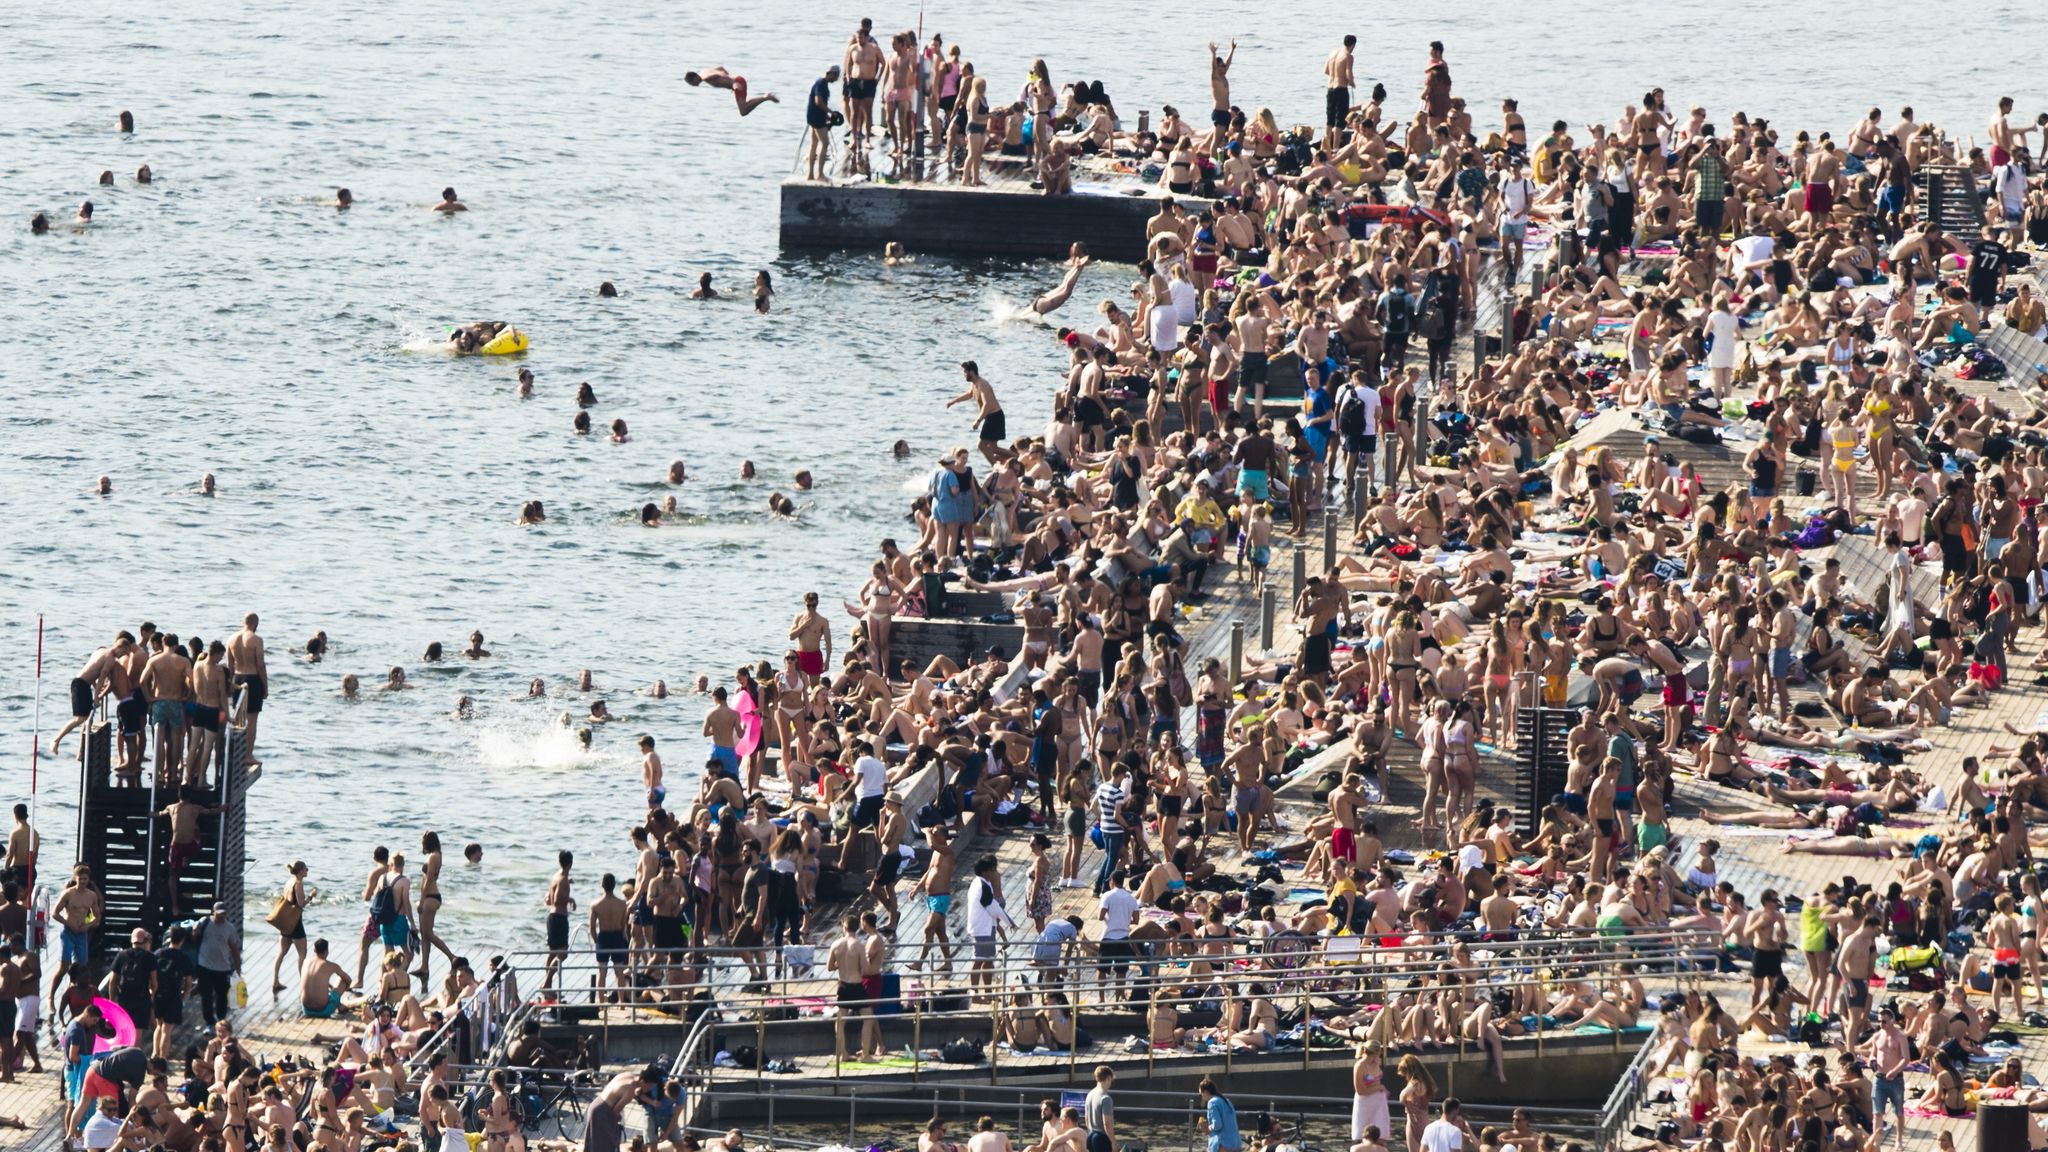
\includegraphics{sorenga.jpeg}
\caption{title}
\end{figure}


    % Add a bibliography block to the postdoc
    
    
    
    \end{document}
